\part{A chacun sa culture qui fait rêver}
\chapter{Le Brésil}

\begin{center}
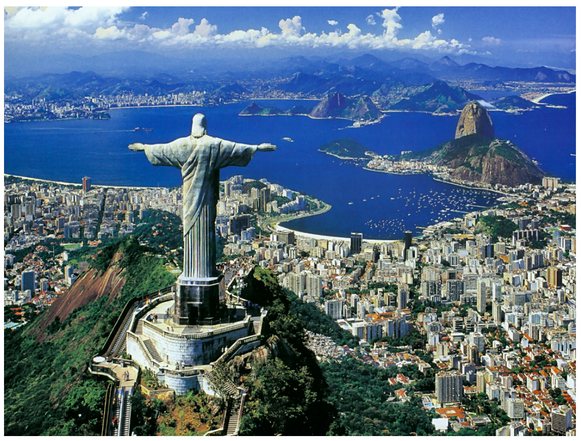
\includegraphics[scale=0.5]{bresil1.png}
\end{center}

\section{Une présentation sommaire}
\paragraph{}
En	juillet	dernier,	je	mettais	les	pieds	en	Amérique	du	Sud	pour	la	seconde	fois	de mon	existence.	Après	la	Colombie,	le	Brésil.	La	période choisie	était	plutôt	atypique puisque	j’étais	arrivé	à	Rio	de	Janeiro	deux jours	avant	la	fameuse	victoire	de l’Allemagne	sur	le	pays	hôte.	Un match	que	j’avais	d’ailleurs	pu	suivre	sur	le	sable	de	Copacabana. Jusqu’à	la	mi-temps.	Une grande	partie	de	la	foule	brésilienne	refusa	la	douche	tiède	après	la	froide	et	rentra	chez	elle.
\paragraph{}
Dans	la	culture	moderne,	on	associe	très	rapidement	taxi	avec	New	York.	Merci Hollywood.	Néanmoins,	je	doute	que	leurs	chauffeurs	soient	aussi passionnants	que	ceux	que	l’on	peut	trouver	au	Brésil.	Le	chauffeur	de taxi	brésilien	peut	être	très	causant,	très	aimable	et	faire	figure d’excellent	ambassadeur	pour	son	pays.

\section{Un pays de contrastes}
\paragraph{}
Le	Brésil	est	un	pays	de	contrastes.	Ce	sont	ses	influences européennes, africaines,	et	bien	évidemment	amérindiennes	qui,	depuis	1822,	ont contribué	à	modeler	le Brésil	actuel.	Quel	autre	pays	au	monde	peut	se targuer	de	posséder	une	diversité culturelle	si	riche?
\paragraph{}
Plus	surprenant	par	contre,	l’attention	presque	obsessionnelle	que	portent	certains Brésiliens	à	leur	corps,	opposé	à	d’autres	qui	s’ouvrent	une	voie royale	vers	un diabète	de	type	2.	Le	contraste	est	particulièrement saisissant	lorsque	vous	vous promenez	sur	le	trottoir	qui	sépare	la	plage de	Copacabana	de	l’Avenida	Atlântica. En	effet,	athlètes	avertis	et	obèse se	mélangent	volontiers	sur	ces	quelques	4,5	km de	pavés	noirs	et	blancs. Mais	pour	différentes	raisons.	Les	premiers,	à	pied	ou	à	vélo,	viennent ici	pour	se	dépenser	et	sculpter	leur corps,	mais	cela	est	normal dans	une	ville	où	le	bikini	est	à	la	mode	de	janvier	à	décembre.	En	plus,	la ville	de	Rio	de Janeiro	développe	depuis	2010	un	concept	plutôt original matérialisé	par	la présence d’une	quarantaine	d’instruments	de	musculation	le long	de	ses	plages.	Les	autres,	les	bons	vivants,	se	baladent	à	un rythme plus	décontracté	et	n’hésitent	pas	à	se	laisser	tenter	par	les gourmandises	proposés	par	les	dizaines	de	bars	circulaires	qui	jonchent les	abords	de	la	plage.
\begin{center}
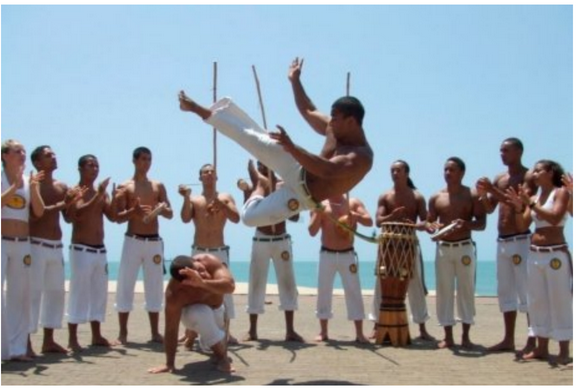
\includegraphics[scale=0.5]{bresil2.png}
\end{center}

\section{Une tradition culturelle}
\paragraph{}
La	tradition	culturelle brésilienne est	extrêmement	riche	et	variée	grâce	à	son	fort métissage,	notamment	du	point	de	vue musical (samba, bossa	nova, forró, frevo...),	chorégraphique	(capoeira)	et culinaire (churrasco,feijoada, caipirinha, guarana...), mais	aussi	sur	le	plan	religieux	(candomblé)	et mythologique.
\paragraph{}
Le	candomblé est	une	des	religions	afro-brésiliennes	pratiquées	au	Brésil,	mais également	dans	les	pays	voisins	tels	que	l'Uruguay,	le	Paraguay, l'Argentine	ou encore	le	Venezuela.	Mélange	subtil	de	catholicisme,	de rites	indigènes	et de croyances	africaines,	cette	religion	consiste	en	un culte	des	orixás,	les	dieux	du candomblé d'origine	totémique	et	familiale, associés	chacun	d'entre eux	à un élément	naturel	(eau,	forêt,	feu,	éclair, etc.).	Se	basant	sur	la	croyance	de	l'existence	d'une	âme	propre	à la nature.
\begin{center}
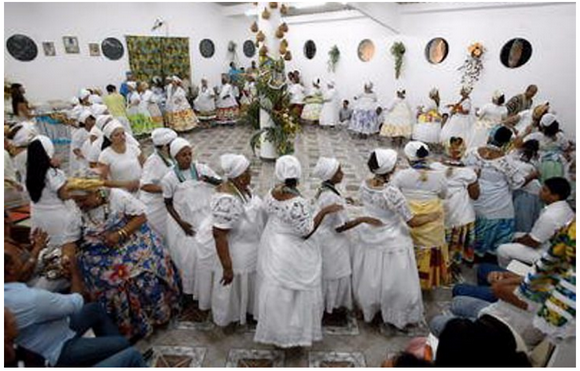
\includegraphics[scale=0.5]{bresil3.png}
\end{center}
\paragraph{}
Les	danses	brésiliennes	sont	très	entraînantes	aussi.
\paragraph{}
Elle	est	reconnue	dans	le	monde	comme	un	symbole	du	Brésil	et	du carnaval	brésilien.	Considérée	comme	l'une	des	expressions	les	plus	cultes du	Brésil,	la	samba	fait	partie	de	l'identité nationale	brésilienne.
\paragraph{}
La	samba	est	un	style	local	au	sud	et	nord	du	Brésil,	en	particulier	à Rio	de	Janeiro, São	Paulo,	Salvador	et	Belo	Horizonte.	Son	importance dans	la	musique	brésilienne	traverse	toutes	les	régions	du	pays,	cependant, des	écoles	de	samba,	musiciens	de samba	et	organisateurs	de	carnaval centrés	sur	la	performance	de	la	samba	se situent	partout	dans	le	pays.

\chapter{Le Japon à travers les animes et les mangas}

\chapter{Le Japon : Matsuris et Croyances}
\section{Les croyances ...}
\paragraph{}
Le Japon ne possède pas de religion particulière. En effet, les japonais auront tendance à se considérer comme appartenant à aucune religion ou à plusieurs religions en même temps. Les religions principales sont le shintoïsme et le bouddhisme mais il y a une minorité de chrétiens et de musulmans. 
\paragraph{}
Ce mélange de religion est possible grâce aux caractéristiques des religions principales du pays. Le shintoïsme est une religion polythéiste tandis que le bouddhisme correspond plus à une philosophie de vie accompagnée de méditation.
\paragraph{}
« On dit souvent que le Japonais naît, grandit et s’amuse shinto, s’éduque confucéen, se marie chrétien, vit dans l’irréligion et meurt bouddhiste ». (Le Japon des Japonais par Philippe PONS et Pierre-François SOUYRI)

\section{... à l'origine des matsuris}
\paragraph{}
Le shintoïsme et le bouddhisme sont à l’origine de nombreuses fêtes traditionnelles autrement appelées Matsuri. En effet, pour attirer la bienveillance des dieux, chacun d’entre eux est prié et vénéré lors de rituel et de fête. Bien que les japonais ne croient pas vraiment en ces dieux, ils accomplissent ces rituels au cas où les dieux existeraient et retireraient leur bienveillance envers les japonais.
\paragraph{}
Ces fêtes ont lieu régulièrement tout au long de l’année. Au printemps, les Japonais fêtent le repiquage du riz et prient pour se protéger des épidémies. En été, ils prient pour se protéger contre les typhons et les ravages causés par les insectes ainsi que pour leurs ancêtres.  En hiver, ils prient pour la nouvelle année. Il y a aussi des fêtes locales pour prier les dieux locaux à différents moments de l’année. 
\paragraph{}
Lors de ces festivités, les hommes défilent dans le quartier en portant le mikoshi (sorte d’autel portatif) sur leurs dos. Ils sont vêtus d’un happi (veste découvrant leurs torses) et d’un fundoshi (sorte de cache-sexe traditionnel). Une fois l’autel retourné au temple, la fête continu le long de la rue du temple où l’on peut trouver des stands de friandises en sucres, de nouilles sautées, de porte-bonheurs… 
\begin{center}
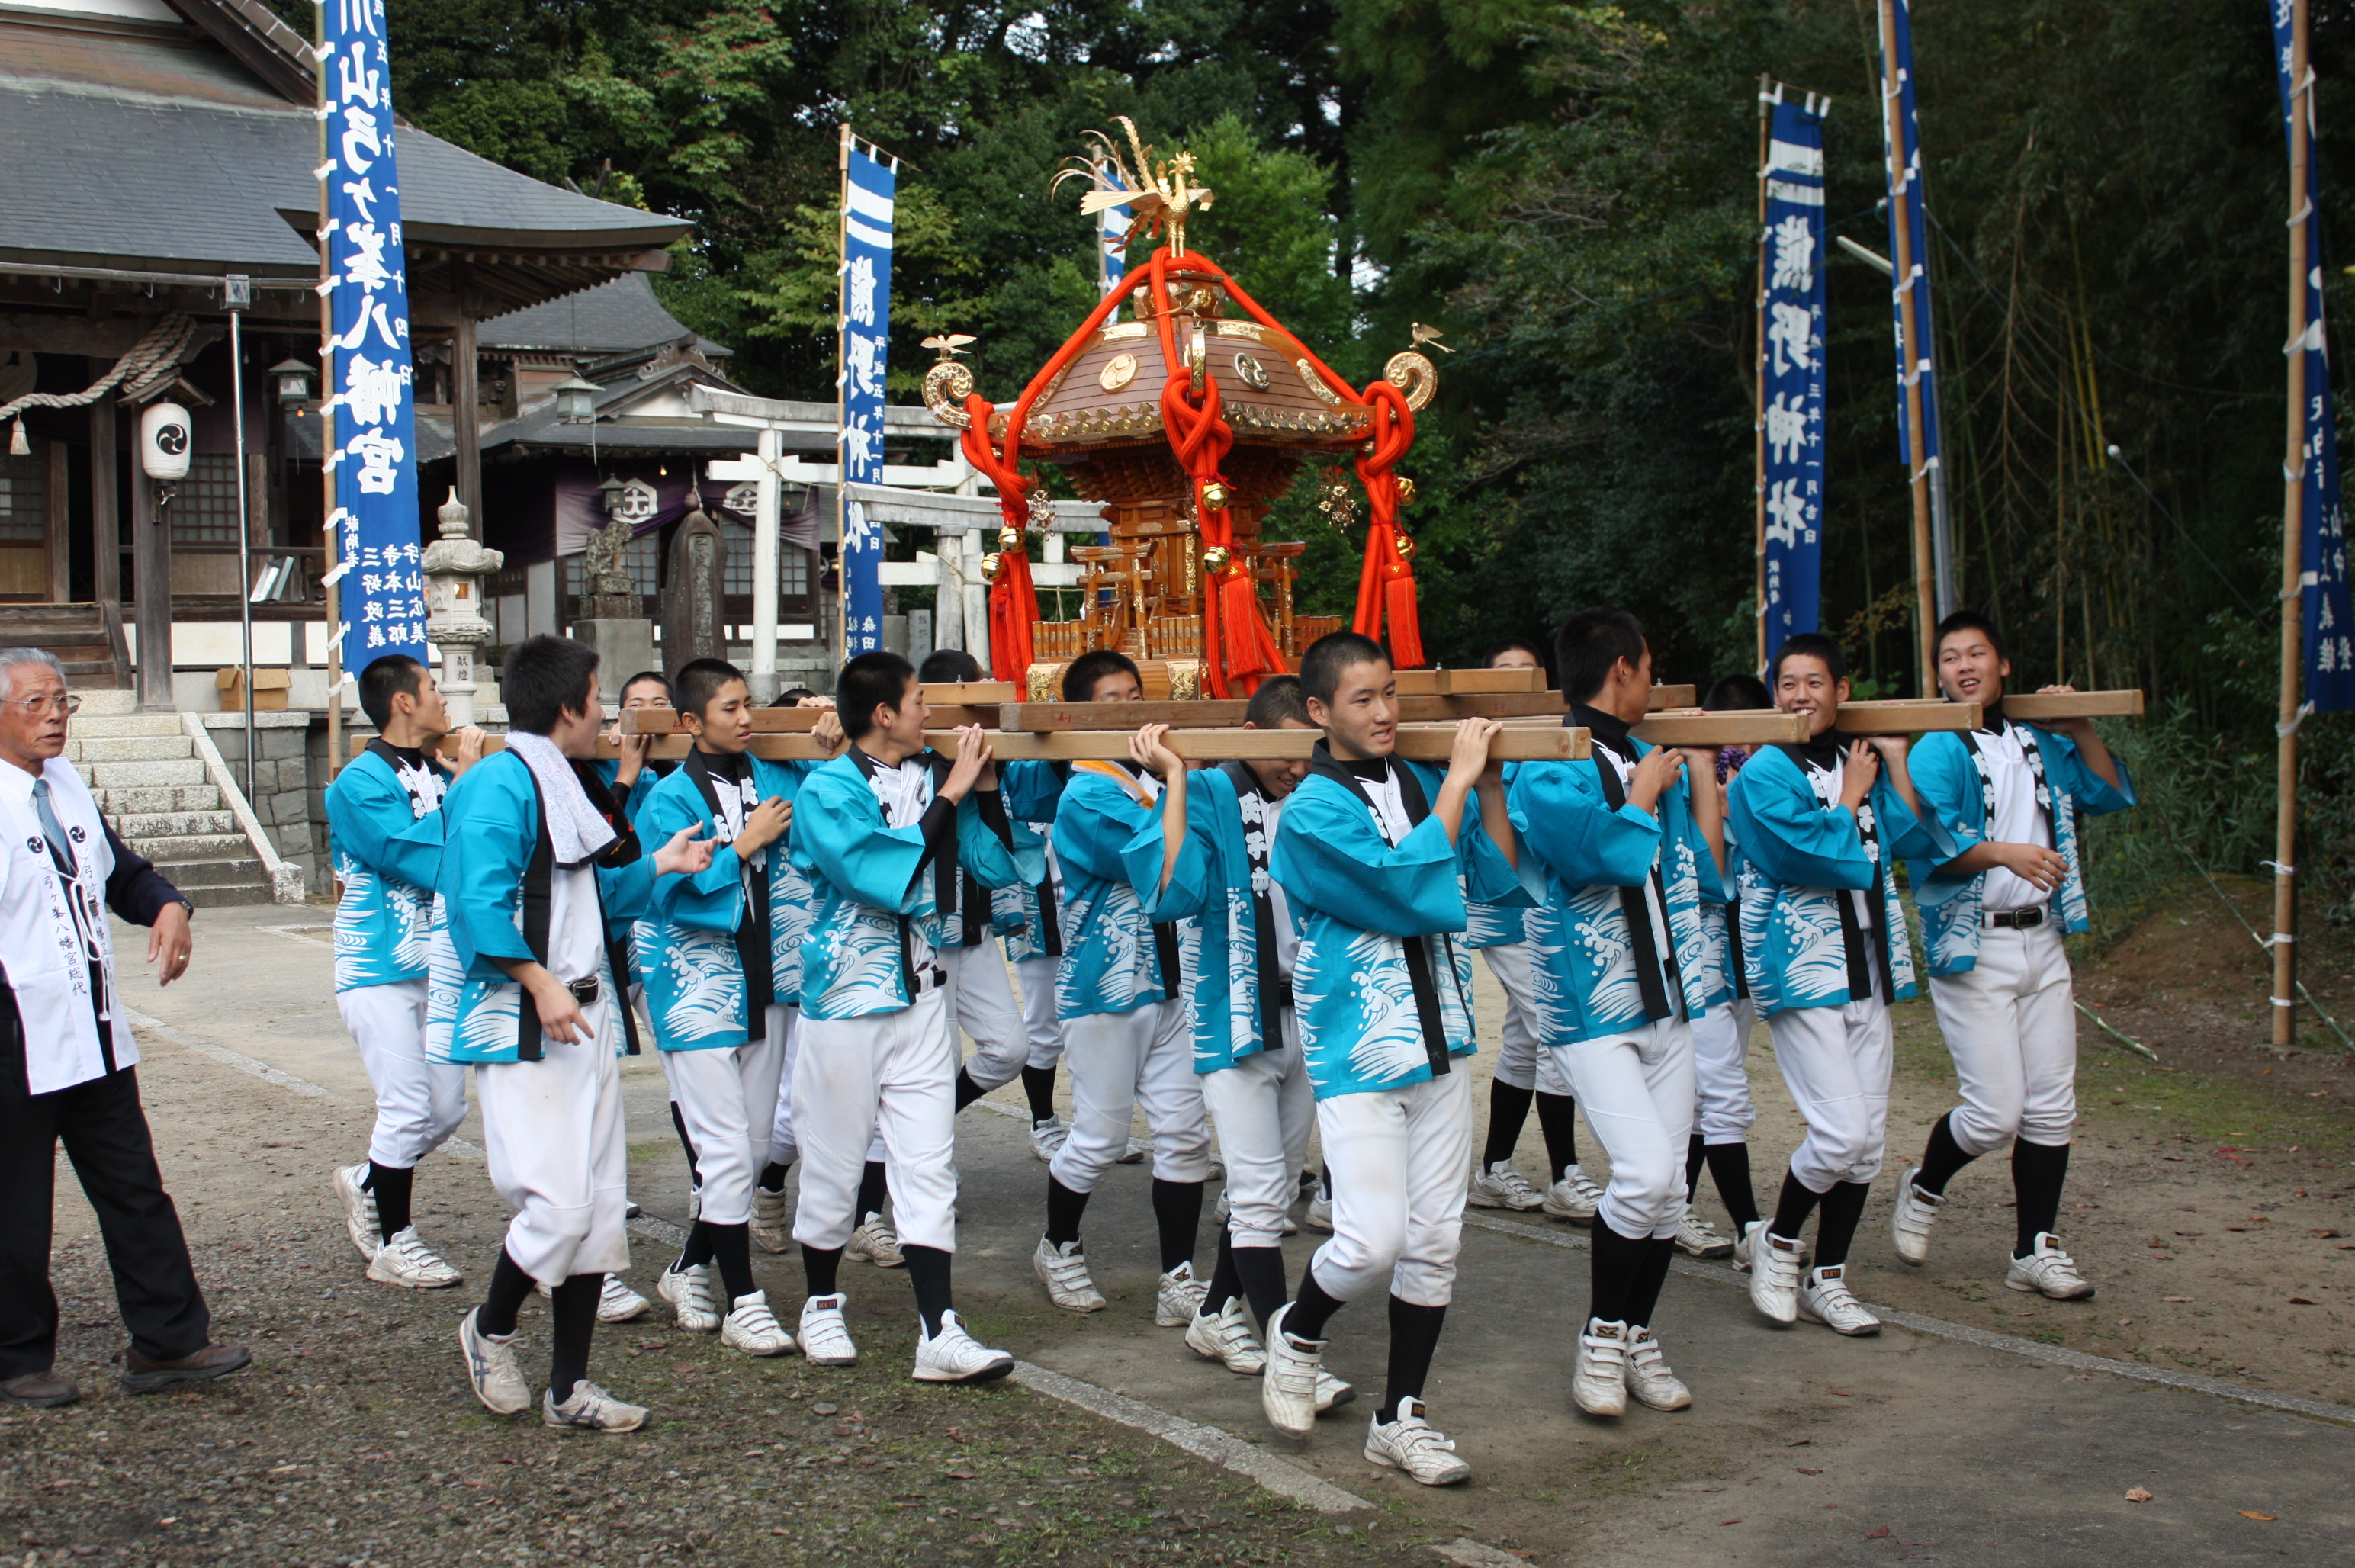
\includegraphics[scale=0.07]{mikoshi.jpg}
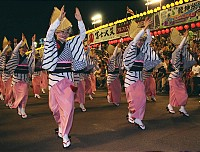
\includegraphics[scale=1.3]{odori.jpg}
\end{center}
\paragraph{}
Dans les plus grands matsuris, de grands chars défilent à travers le quartier accompagnés des flûtes, tambours et gongs. Ces chars sont aussi accompagnés de troupes de danseurs. Les filles profitent de ces festivals pour sortir leurs kimonos pour rentrer dans l’ambiance de la fête.
\begin{center}
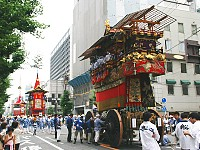
\includegraphics[scale=1.3]{gion.jpg}
\end{center}
\newpage
\section{Les matsuris les plus connus}
\begin{itemize}
\item Aoi matsuri, 15 mai, Kyoto
\item Aomori nebuta matsuri, 2-7 août, Aomori
\item Awa-Odori, 12-15 août, Tokushima
\item Danjiri matsuri, deuxième week end de septembre, Kishiwada
\item Etchu owara kaze no bon, 1-3 septembre Toyama
\item Gion matsuri, juillet, Kyoto quartier de Gion
\item Gozan no Okuribi, 16 août, Kyoto
\item Hadaka matsuri, troisième samedi de février, Okayama
\item Hakata Gion Yamakasa, 1-15 juillet, Hakata
\item Ise-jingu kannamesai et ninamesai, 15-25 octobre et 23-29 novembre, Ise
\item Jidai matsuri, 22 octobre, Kyoto
\item Kanda Matsuri, deuxième dimanche de mai, Tokyo
\item Namahage, 31 décembre, Oga
\item Narita-san setsubun-e, 3 février, Narita
\item Onbashira, avril tous les six ans, Suwa
\item Otaue matsuri, 14 juin, Osaka
\item Sanja matsuri, troisième week end de mai, Tokyo
\item Sanno matsuri, 14-15 avril, Takayama
\item Sendai Tanabata matsuri, 6-8 août, Sendai
\item Sentei-sai, 3-4 mai, Shimonoseki
\item Festival de la neige de Sapporo, mi-février, Sapporo
\item Tenjin matsuri, 24-25 juillet, Osaka
\item Yosakoi matsuri, 9-12 août, Kochi
\end{itemize}

\chapter{Les elfes}